Unlike Python, all Scheme lists are linked lists. Recall a linked list is made up of Links that have a first and a rest, where the rest is another Link. Similarly, Scheme lists are made up of pairs with a first and a rest, where the rest is another pair.

\textbf{Ways to make scheme lists:}
\begin{itemize}
\item Cons \\
\textbf{Syntax:} \lstinline{(cons <car-elem> <cdr-elem>)} \\
Takes in a pair of two elements; similar to how a python linked list has 2 elements as well- first and rest
\item List \\
\textbf{Syntax:} \lstinline{(list <elem1> <elem2> ...)} \\
Takes in an arbitrary number of elements/arguments, and constructs a list where each elem is the first of its own pair. Note how this differs from \lstinline{cons} where you specify a first and rest rather than just specifying the first of each pair. All the arguments will be evaluated before being collected into the scheme list.
\item ' (aka single quote) \\
\textbf{Syntax:} \lstinline{'(<elem1> <elem2> ...)} \\
Also takes in an arbitrary number of elements and construct a list out of the elements, but the arguments are not evaluated.
\end{itemize}
Example:
\lstinline{(cons 1 (cons 2 (cons 3 nil)))} = \lstinline{(list 1 2 3)} = \lstinline{'(1 2 3)}
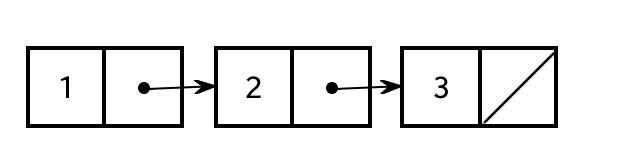
\includegraphics[scale=0.6]{scheme_list}

\textbf{Ways to access list items:}
\begin{itemize}
\item Car \\
\textbf{Syntax:} \lstinline{(car <pair>)} \\
Gets you the first item of a pair
\item Cdr \\
\textbf{Syntax:} \lstinline{(cdr <pair>)} \\
Gets you the second item of a pair
\end{itemize}
\begin{itemize}
\item Cadr \\
\textbf{Syntax:} \lstinline{(cadr <pair>)} \\
Gets you the \lstinline{car} of the \lstinline{cdr}
\end{itemize}
\begin{itemize}
\item Cddr \\
\textbf{Syntax:} \lstinline{(cddr <pair>)} \\
Gets you the \lstinline{cdr} of the \lstinline{cdr}
\end{itemize}

\begin{guide}
\begin{blocksection}
\textbf{Teaching Tips}
\begin{itemize}
  \item Emphasize to students that Scheme lists are linked lists and NOT Python lists
  \begin{itemize}
    \item Discuss the limitations (e.g. no indexing) and capabilities (e.g. recursion)
  \end{itemize}
  \item If you're an old bear\textsuperscript{TM}, keep in mind that dotted lists have been removed from the curriculum, so Scheme lists have the same functionality as linked lists
  \begin{itemize}
    \item \lstinline{(cons 1 2)} will now raise a SchemeError instead of creating a Malformed list
  \end{itemize}
  \item The \href{https://code.cs61a.org/}{61A Scheme Web interpreter} is \textbf{very useful} for visualizing lists!
  \item If you choose to give a mini-lecture on Scheme list syntax, try using each keyword in an example instead of just talking about them!
\end{itemize}
\end{blocksection}
\end{guide}
